\section{Safe Collection Model}
\label{sec:architecture}

%%%%%%%%%%%%%%%%%%%%%%%%%%%%%%%%%%%%%%%%%%%%%%%%%%%%%%%%%%%%%%%%%%%%%%%%%%%%%%%%%%%%%%%
% Intro to arch
%%%%%%%%%%%%%%%%%%%%%%%%%%%%%%%%%%%%%%%%%%%%%%%%%%%%%%%%%%%%%%%%%%%%%%%%%%%%%%%%%%%%%%%

To address the concerns outlined in the previous section we introduce two
new abstractions: safe collections, an abstraction that encapsulates
a dataset and the set of policies that govern its use; and stewards, privileged users
to manage safe collections while separating management of data from infrastructure.
In this model, administrators first define a safe collection and declare one
or more stewards to manage that collection. This process transfers
all administrative responsibilities regarding access to, and export of, data to the stewards.
%who now take ownership and responsibility for the safe collection.

\subsection{Safe Collections}

Selecting the policies, protocols, infrastructure, and
software settings to ensure that individual datasets are adequately secured requires consideration
on a case-by-case basis.
%To represent these policies, such that dataset owners can manage these considerations,
%we define safe-collections.
Safe collections enable system administrators to partition the key administration
aspects of managing the relationship between data and users (e.g., analysts who use that data).
Safe collections encapsulate the data-store in which a dataset resides, and a consistent set of policies
that controls access to that dataset.

Safe collections are defined with policies that govern limits as well as access to, and use of,
data in that collection. They specifically regulate access, usage, and data export.
The policies supported by safe-collections are as follows:

\textbf{SecurityClass:} A binary classification that specifies the constraints
on accessing data in that collection. Setting to \texttt{Public} means that the data is freely
(but securely) accessible to a set of permitted users and no other
data administration policies can be set.  Setting to \texttt{Private}
requires that safe collection policies are set.

\textbf{Classification:} Categorizes the type of data stored in the
safe collection including specifying that the data is controlled by
a license or that the data is subject to regulations (e.g., HIPAA or FEDRAMP).
This information is used by stewards and administrators when
managing a safe collection.

\textbf{StewardGroup:} Defines the user(s) who are permitted to
administer the safe collection. These users are subsequently
allowed to modify policies and are tasked with managing the
security of data within the collection.

\textbf{ReadAccess:} A set of policies that define who can
access data, under what conditions, and for what period of time.
Policies can define individual users or groups of users, particular
authentication requirements (e.g., using two factor authentication),
and for arbitrary periods of time from days to years.

\textbf{ExportControl:} Specifies policy on export of derived or copied data
from safe collection such as steward review process.

\textbf{LinkControl:} An advanced policy that permits
or prohibits datasets within a safe collection being
combined. This is an important control as some datasets
are intentionally split and linking restricted for purposes
of deidentification or anonymization .



%% Public data
%Public datasets are assumed to contain no sensitive content and thus do not require access control nor
%export control. Setting \texttt{SecurityClass} to \texttt{Public} indicates that the safe-collection does
%not require a Steward and that all authenticated users on \NAME may access this dataset. None of the added
%security features of safe-collections need apply.
%
%% Common features for private data
%Confidential and regulated datasets both require \texttt{SecurityClass} to be set to \texttt{Private}
%and require that a steward group is specified. In addition, constraints can be set on the duration
%for which analysts could be granted access. This ensures that access privileges expire and require
%re-evaluation of the scope and nature of the analyst's work before access is extended. To limit the risk of
%re-identification in datasets that contain anonymized data the safe-collections allow for whitelisting and
%blacklisting other safe-collections. Job submissions to \NAME are checked for data requests that have
%linkage conflicts, and denied at submit time.
%\yadu{Linkage feature pending}
%
%% cite garfinkel for de-identification risks
%Safe-collections that contain regulated datasets often require oversight to ensure that all computed results
%are inspected and approved by a steward before export. This is enforced by setting the
%\texttt{ExportStewardApprovalReqd} flag.
%Analysis results from tasks that consumed data from any safe-collection with this flag has all of the
%results posted back to the same safe-collection, thus inheriting the same privileges as the source.
%% worker roles are granted write privileges to the outputs section of a safe-collection
%As a result, only stewards can view the results and export to a public safe-collection. Since results are
%stored within the parent safe-collection, users can apply analysis operations on results without oversight,
%and only request for export of the final results of a deep analysis pipeline.

\subsection{Stewardship}

% Why do we have them / inital role
%As that number of datasets managed by \NAME increase it is crucial that administrative
%tasks are distributed to individual collection administrators.

Safe collection stewards are a specialized role that aims to separate
concerns from those that operate \NAME and those that manage the data stored in \NAMENS.
Stewards play a management role in evaluating the disclosure risks associated with a
dataset and codifying the security protocols protecting the safe collection.
Thus, for datasets with particular data use agreements or restrictions, they
are responsible for ensuring all requirements are met. In the event of a
data breach or data loss, they are responsible for following appropriate
mitigation plans.

Stewards are responsible for activities such as approving access to a collection, reviewing
export requests, and managing policies on the collection.
As described above, stewards are pre-associated with a particular safe collection by
way of a specialized role and mapping to a collection's storage layer.
External users (e.g., analysts) can discover
and then obtain access to safe collections by listing available safe collections and requesting
access to individual collections.
Stewards for a safe collection are presented with a list of user requests and must explicitly approve access
for a specific duration. Throughout the duration of a user's access to a collection
stewards may review their actions and revoke access at any time. When users attempt
to export data from an export controlled safe-collection, the data is not immediately
accessible to the user. Rather, the exported data is collected and stored privately
assuming that it contains microdata, and is released pending review by a a steward.


\subsection{User Flows}

Here we describe the two most common flows introduced by the safe collection model:

\subsubsection{Access Flow}

Bob, an analyst, authenticates to \NAME and requests access to a private safe collection.
The request is added to the stewarship dashboard and is visible to all stewards
of that collection. Alice, a steward for the requested
safe collection views and then approves Bob's request for a period of $n$ days.
The approval process adds the appropriate policies to the
safe collection granting access to Bob. Bob now can submit analysis tasks through the various
interfaces offered by \NAME, that specify data items from the safe collection as inputs.
The REST API marks the analysis task as export controlled since it draws results
from an export controlled safe collection.
The submitted task is posted to an internal queue from which a
worker node in the \NAME private subnet picks up Bob's task. The worker node assumes Bob's identity and with
his credentials requests data from the safe collection. Since Bob now has read privileges for the
safe collection, the data is fetched to the worker node, on which the analysis task is executed.
Upon completion, the worker node puts the generated results in the export-controlled
output directory of the safe collection as the task used export controlled data.
Bob's analysis is now complete, but he is unable to view the
results as they require steward approval. This flow is show in \figurename~\ref{fig:flow1}

\begin{figure}
  \center
  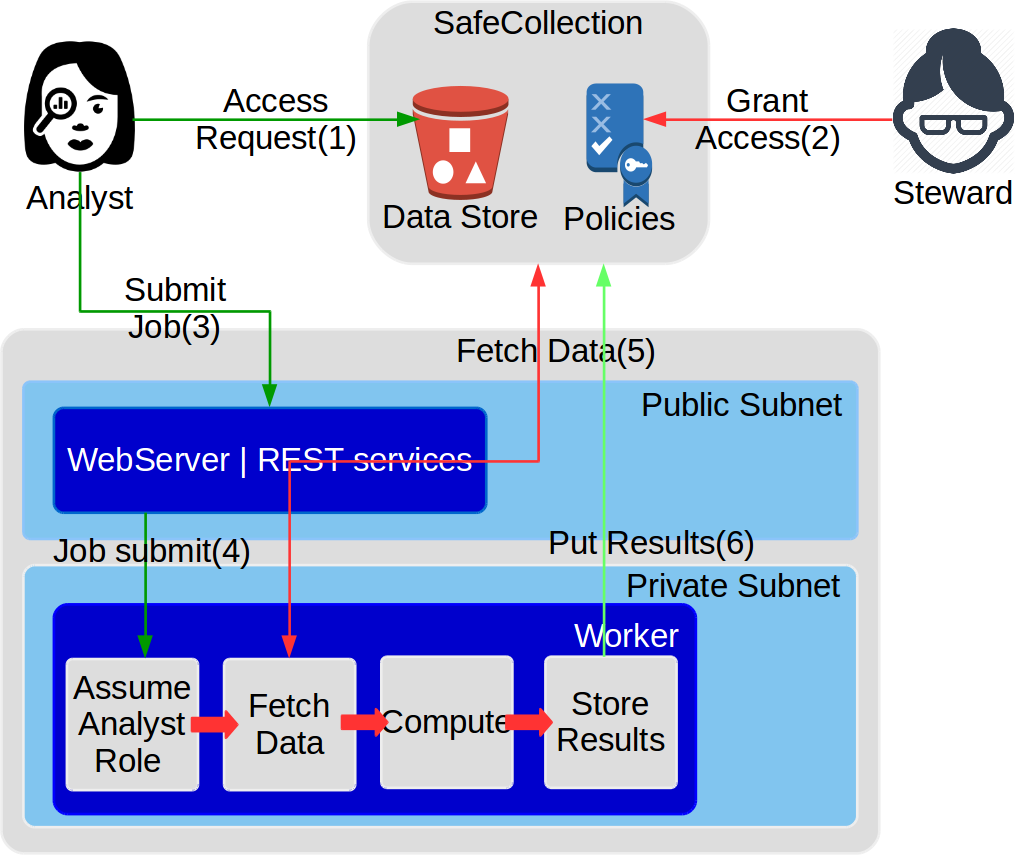
\includegraphics[width=0.45\textwidth]{figures/safe_flow.png}
  \caption{Safe collection schema}
  \label{fig:flow1}
  \vspace{-1.5em}
\end{figure}


\subsubsection{Export Flow}

Once Bob's analysis task is complete Bob realizes that he requires export approval before he may view the
results, so he issues a request to export his results. Alice, one of the collection's stewards, recieves
the export request on her dashboard. Alice assumes
the steward role with a fresh authenticated token, and accesses the results and the complete description
of Bob's analysis task. Alice reviews the data and the analysis to determine if the results are
safe for export. When she is satisfied with Bob's process, she initiates data export. \NAME
uses Alice's temporary credentials to transfer the results from the safe collection to a public
safe collection, accessible only to Bob, and updates the task information with new location of the results. Bob can now log on
and view or download the results. This flow is show in \figurename~\ref{fig:flow2}

\begin{figure}
  \center
  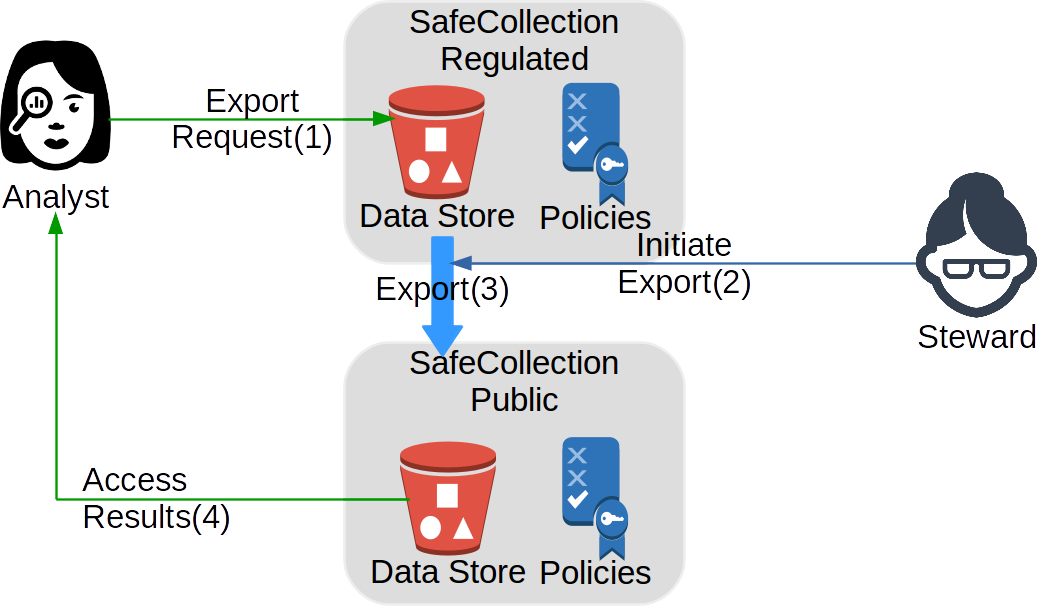
\includegraphics[width=0.45\textwidth]{figures/export_flow.png}
  \caption{Safe collection schema}
  \label{fig:flow2}
  \vspace{-1.5em}
\end{figure}


\begin{figure*}%[ht]
  \center
  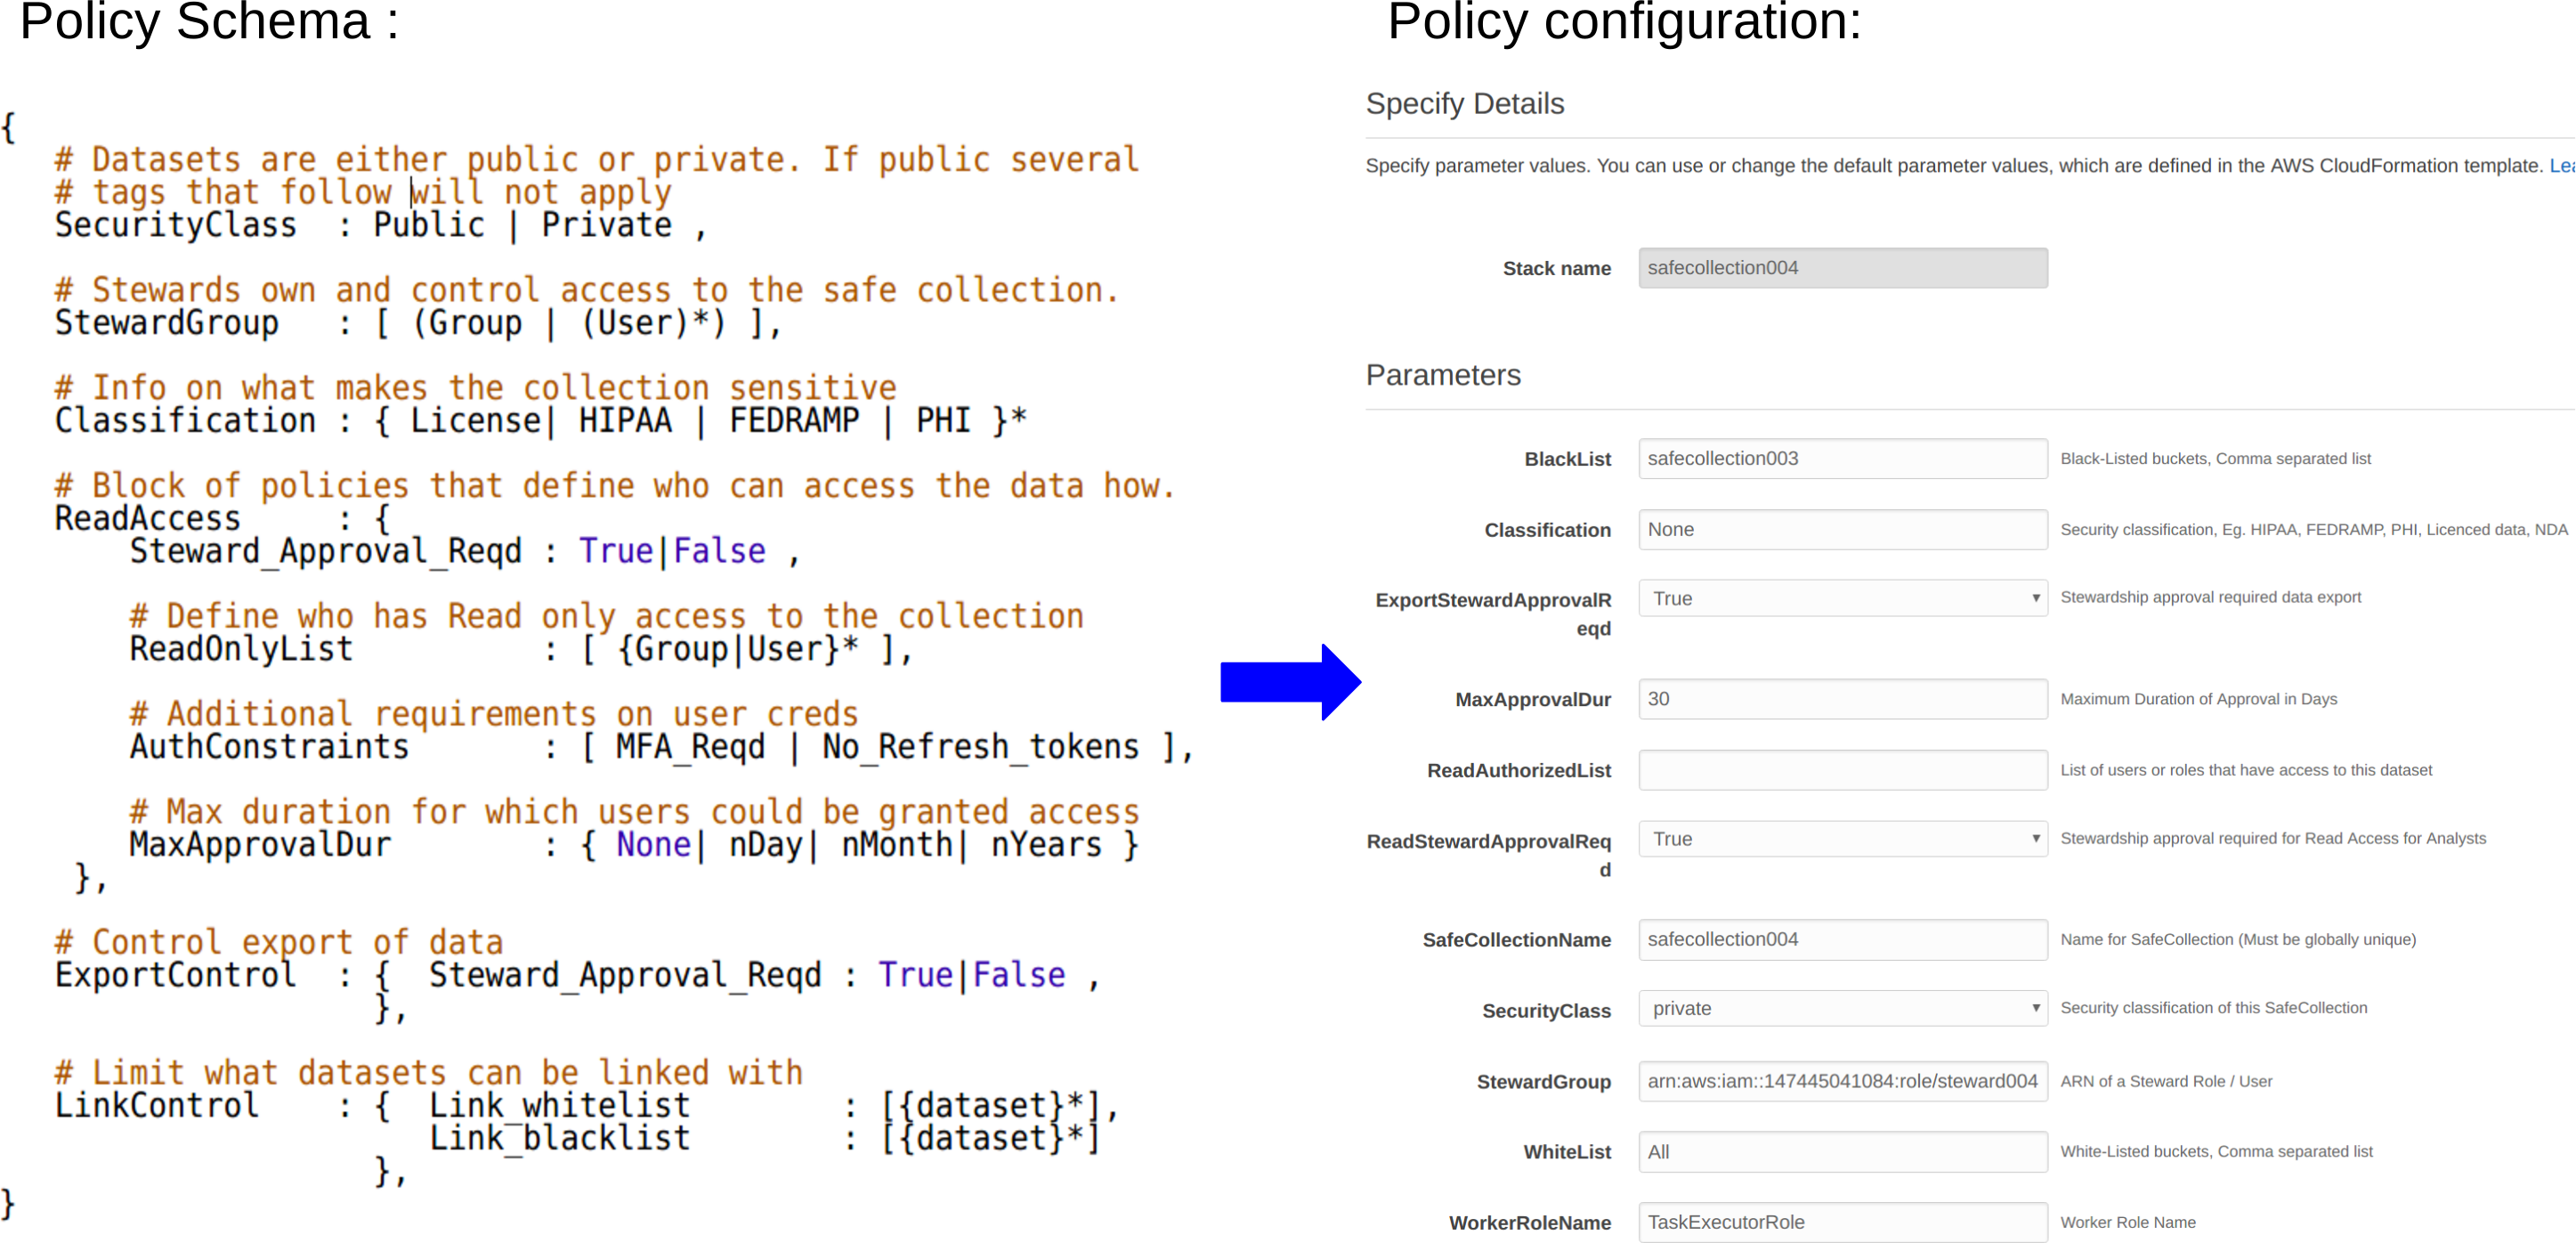
\includegraphics[width=\textwidth, height=8cm]{figures/meta-policy.png}
  \caption{Meta-policy specification and configuration}
  \vspace{-1.5em}
  \label{fig:schema}
\end{figure*}

\section{Implementation}

The \NAME service is built upon a set of reliable and secure
AWS services. We extend this architecture to support safe collections
by building upon additional AWS capabilities and services.

Safe collection policies are expressed on \NAMENS's managed
data via AWS Identity and Access Management (IAM) policies
and S3 bucket policies.
A safe collection is described in CloudFormation templates, where
CloudFormation provides a reproducible method for instantiating infrastructure
based on a standard JSON description. For example, it defines
the S3 bucket, bucket policies granting exclusive administrative privileges to a steward role,
and IAM policies granting appropriate privileges to cloud kotta worker machines to store analysis results.
%This allows safe-collection descriptions to be verifiable, reproducible, and shareable.

To enable the definition and management of safe collection policies we
rely on a meta-policy model. The meta-policy model enables specification
of the policies described above. Each safe collection is associated with a steward
(or group of stewards) who may manage the collection's policies. To simplify use, the meta-policy schema
is translated to a web-based form that can be completed by administrators during the creation of a safe collection.
The defined policies (from the form or otherwise) is stored as a set of secure tags
on the collection's data storage bucket. The schema is enforced by the various services that interact
with the safe collection. The schema and the generated form are shown in \figurename~\ref{fig:schema}



Upon creation of a safe collection a single steward group (implemented as an IAM role) is added to the
access policies of the safe collection. This steward role is the sole entity on the platform capable of
updating policies attached to the safe collection.
Multiple users can be associated with the steward role---this is often recommended such
that requests can be served quickly.
Having established one's identity (via the \NAME authentication workflow) users
may ``assume'' a privileged IAM role for which they are permitted.
When assuming the steward role, a user temporarily gains the privileges to carry out operations such
as updating access policies and approving the export of data from a safe collection.

% implementation of access control
Access control on safe collections are managed by stewards. Access privileges for specific users
are granted, extended, and revoked via S3 bucket policies. At the time of creation all
privileges over bucket policies are granted to the steward and revoked for all other entities. This
guarantees that only the stewards can grant privileges on a safe collection. Access to other users
is granted by stewards by adding a new bucket policy conditional on an expiration deadline. These policies may be revoked or
extended by updating the expiration deadline, thus offering fine-grained control to stewards for managing
access.

Data derived from safe collections (e.g., results from tasks that consumed data from that collection)
are stored in the same safe collection, thus inheriting the same policies as the safe collection itself.
As a result, only stewards can view the derived data and determine if it is safe to
export the data
Stewards have complete visibility over all data that was used as input to an analysis as
well as the operations (analysis steps) made by the analysts to derive their results.
It is therefore possible to trace the entire provenance of the derived data from an
analysis pipeline since all analysis tasks are logged.
If an export request is approved, data is copied from the host collection to a public safe collection.
It is important to note that even public safe collections have server side encryption and
are only accessible to authenticated users via temporary signed URLs.
As derived data are stored within the parent's safe collection, users can continue
to perform analysis operations on results without oversight,
and only request export of data that must leave the safe collection (e.g., the
final results of a deep analysis pipeline).

Export approvals are implemented as copy operations between buckets. This usually is a copy from a
private safe-collection to a public safe-collection's bucket.
\NAME ensures that the export operation is consistent with the policies established for the originating
safe collection.


%On export controlled safe-collections, results generated by analysis tasks on \NAME are not visible to the
%analysts until approved by a Steward. This is implemented by having workers write all results to the
%parent safe-collections output directory and thus inheriting the same security privileges of the parent.
